\documentclass{article}

% For figure formatting
\usepackage{float}

% For code formatting
\usepackage{listings}
\lstset{
    basicstyle=\ttfamily,
    columns=fullflexible,
    keepspaces=true,
    showspaces=false,
    showstringspaces=false
}

% For syntax highlighting
\usepackage{xcolor}

% Language setting
% Replace `english' with e.g. `spanish' to change the document language
\usepackage[utf8]{inputenc}        % Support UTF-8 encoding for Vietnamese
\usepackage[vietnamese, english]{babel} % Enable both English and Vietnamese
\usepackage[T5]{fontenc}           % Support Vietnamese characters properly

% Set page size and margins
% Replace `letterpaper' with `a4paper' for UK/EU standard size
\usepackage[letterpaper,top=2cm,bottom=2cm,left=3cm,right=3cm,marginparwidth=1.75cm]{geometry}
\usepackage[utf8]{inputenc}
\usepackage{setspace}  % Import setspace package

\doublespacing  % Apply 1.5x line spacing globally

% Useful packages
\usepackage{amsmath}
\usepackage{graphicx}
\usepackage[colorlinks=true, allcolors=blue]{hyperref}

\title{LYE - Learning Yocto Embedded}
\author{Nhat-Trieu Huynh-Pham}

\begin{document}
\maketitle

\begin{abstract}
This document provides an overview of my journey to learn \textbf{Yocto Project} from the ground up, covering key concepts, development workflows, and practical insights gained along the way.
\end{abstract}

\section{Introduction}

The history of the \textbf{Yocto Project} begins with the need to create a coherent and flexible environment for building software for embedded devices that could support a diversity of hardware architectures and application requirements. Over the years, the Yocto Project has gained broad recognition and support in the industry, becoming the standard for creating custom operating systems for a wide range of devices, from simple gadgets to sophisticated industrial and commercial customized systems.

The \textbf{Yocto Project} is not an operating system itself, but a set of tools that allow developers to precisely configure, compile, and deploy their versions of Linux, tailored to the specific requirements of their projects. So, as you can see, it is the perfect solution for many embedded developers! \cite{2}

The rest of this document is structured as follows:
\begin{itemize}
    \item \textbf{Section \ref{sec:terms}} introduces essential terms related to the Yocto Project.
    \item \textbf{Section \ref{sec:build-steps}} details the step-by-step process of building a Yocto-based system.
    \item \textbf{Section \ref{sec:customization-examples}} presents some examples of customizing a Yocto build to bring-up/port the \textbf{Raspbery Pi} hardware.
    \item \textbf{Section \ref{sec:final-example}} provides a final example for hands-on practice.
\end{itemize}

\section{Terms} \label{sec:terms}

\subsection{BitBake}
BitBake is the main build tool of Yocto, responsible for processing configuration files and generating OS images. It is similar to Makefile but more flexible.

\subsection{Recipe (Công thức - \texttt{.bb})}
A recipe describes how to compile and install a specific software package. For example, a recipe for \texttt{busybox} specifies how to fetch the source code, compile it, and package it.

\subsection{Layer}
A layer is a collection of recipes, configurations, and patches organized to facilitate management. Examples include:
\begin{itemize}
    \item \texttt{meta-yocto}: The main layer of Yocto.
    \item \texttt{meta-raspberrypi}: A layer supporting Raspberry Pi.
    \item \texttt{meta-custom}: A user-defined custom layer.
\end{itemize}

\subsection{Machine}
The target hardware specification for Yocto, defined using the \texttt{MACHINE} environment variable. Examples:
\begin{itemize}
    \item \texttt{raspberrypi4-64} for Raspberry Pi 4.
    \item \texttt{qemuarm64} for ARM 64-bit emulation.
\end{itemize}

\subsection{Distro (Bản phối)}
A set of policies and configurations that define a specific OS distribution. For example, \texttt{poky} is Yocto's default distribution.

\subsection{Poky}
A reference distribution in Yocto, including BitBake and a set of essential layers. \texttt{Poky} helps create a minimal embedded Linux system.

\subsection{Image (Hình ảnh hệ điều hành)}
The final output of Yocto, containing the kernel, root filesystem, and bootloader. Common image types include:
\begin{itemize}
    \item \texttt{core-image-minimal}: A minimal OS.
    \item \texttt{core-image-full-cmdline}: A full command-line OS.
    \item \texttt{core-image-sato}: A graphical OS.
\end{itemize}

\subsection{SDK (Software Development Kit)}
A toolkit for developing applications for Yocto-based systems. It can be generated using:
\begin{lstlisting}[language=bash]
bitbake -c populate_sdk <image-name>
\end{lstlisting}

\subsection{Toolchain}
Is a set of tools (compiler, linker, debugger) to compile software for embedded systems.

\subsection{devtool}
A rapid development tool in Yocto that allows adding, editing, and testing recipes.

\subsection{Toaster}
Is a web interface to manage Yocto's build system.

\section{Build Steps} \label{sec:build-steps}

\section{Customization examples} \label{sec:customization-examples}

Most of the examples presented in this document are derived from the blog \cite{1}.

\subsection{Hello World}
This section describes how to create a custom layer in Yocto and add a simple \textbf{Hello World} application.
\section{Creating a New Layer}
\subsection{Hello World}

This section describes how to create a custom layer in Yocto and add a simple Hello World application.

\begin{itemize}
    \item \textbf{Create a New Layer:}  
    Run the following command to create a new layer named \texttt{meta-helloworld}:
    \begin{lstlisting}[language=bash]
    bitbake-layers create-layer ../meta-helloworld
    \end{lstlisting}
    This command generates a directory structure for the new layer.

    \item \textbf{Create the Recipe Directory:}  
    Set up the necessary directories for the recipe and source files:
    \begin{lstlisting}[language=bash]
    mkdir -p ../meta-helloworld/recipes-example/helloworld/files
    \end{lstlisting}
    - \texttt{recipes-example/} stores recipes.
    - \texttt{helloworld/} contains the Hello World recipe.
    - \texttt{files/} holds the source code.

    \item \textbf{Add Source Code:}  
    Inside the \texttt{files} directory, create a simple C program:
    \begin{lstlisting}[language=c]
    #include <stdio.h>
    int main() {
        printf("Hello, Yocto!\n");
        return 0;
    }
    \end{lstlisting}
    Save this as \texttt{helloworld.c} inside \texttt{files/}.

    \item \textbf{Create the Recipe File:}  
    Now, create a recipe file named \texttt{helloworld\_1.0.bb} inside \texttt{recipes-example/helloworld/}:
    \begin{lstlisting}[language=bash]
    touch ../meta-helloworld/recipes-example/helloworld/helloworld_1.0.bb
    \end{lstlisting}
    Edit the file and add the following content:
    \begin{lstlisting}[language=sh]
    DESCRIPTION = "Simple Hello World application"
    LICENSE = "MIT"
    SRC_URI = "file://helloworld.c"

    S = "${WORKDIR}"

    do_compile() {
        ${CC} helloworld.c -o helloworld
    }

    do_install() {
        install -d ${D}${bindir}
        install -m 0755 helloworld ${D}${bindir}
    }
    \end{lstlisting}

    \item \textbf{Add the Layer to Yocto:}  
    Register the new layer in the build environment:
    \begin{lstlisting}[language=bash]
    bitbake-layers add-layer ../meta-helloworld
    \end{lstlisting}

    \item \textbf{Build the Recipe:}  
    Run the following command to compile and build the \texttt{helloworld} application:
    \begin{lstlisting}[language=bash]
    bitbake helloworld
    \end{lstlisting}
\end{itemize}

\textbf{Note:} Now you can use \textbf{scp} which enabling the \textbf{ssh} feature to push the file to the board and run the application. Additionally, if you want to ensure that the \texttt{helloworld} application is included in the final image, follow these steps:

\begin{itemize}
    \item \textbf{Modify Local Configuration:}  
    Open the \texttt{local.conf} file inside the build directory and append the following line:
    \begin{lstlisting}
    IMAGE_INSTALL_append = "helloworld"
    \end{lstlisting}

    \item \textbf{Build the Image:}  
    Run the following command to build your image with the included \texttt{helloworld} application:
    \begin{lstlisting}[language=bash]
    bitbake core-image-minimal
    \end{lstlisting}
\end{itemize}

\textbf{Output:} 
    \begin{lstlisting}[language=bash]
    root@raspberrypi4-64:~# which helloworld
    /usr/bin/helloworld
    root@raspberrypi4-64:~# helloworld
    Hello World, I'm from LYE!
    root@raspberrypi4-64:~#
    \end{lstlisting}

\subsection{SPI}
\begin{itemize}
    \item \textbf{Kenrel configuration}
    \begin{itemize}
        \item \textbf{Create a new meta layer} to add updates for kernel changes: \texttt{meta-kernelmodule}.
        \item Enable options in menuconfig:
        \begin{lstlisting}[language=bash]
        bitbake -c menuconfig virtual/kernel
        \end{lstlisting}
        \begin{itemize}
            \item \texttt{\textbf{FB\_TFT\_ILI9341:}} (depends on \texttt{\textbf{FB\_TFT}})
            \begin{figure}[H]
                \centering
                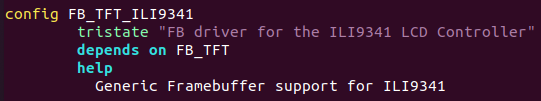
\includegraphics[width=0.5\linewidth]{FB_TFT_ILI9341.png}
                \caption{FB\_TFT\_ILI9341}
                \label{fig:fb_tft_ili9341}
            \end{figure}
            \begin{itemize}
                \item Navigate to \texttt{Device Drivers -> Staging drivers -> Support for small TFT display modules}.
                \item Select \texttt{[*] FB driver for the ILI9341 LCD Controller}.
            \end{itemize}
            \begin{figure}[H]
                \centering
                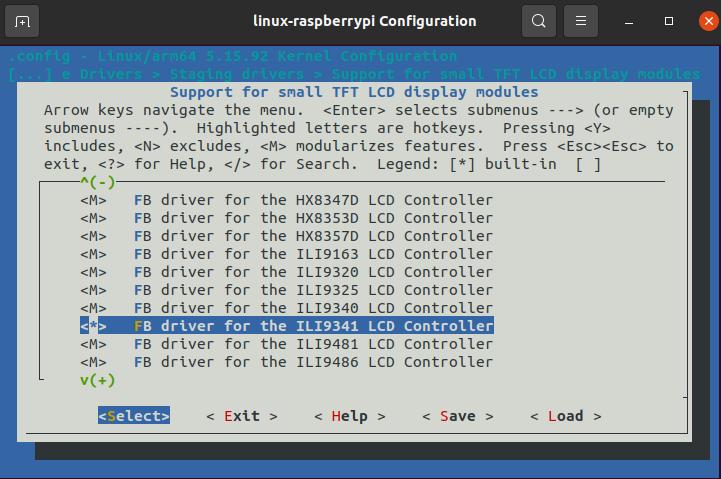
\includegraphics[width=0.5\linewidth]{FB_TFT_ILI9341_menuconfig.png}
                \caption{FB\_TFT\_ILI9341 menuconfig}
                \label{fig:fb_tft_ili9341_menuconfig}
            \end{figure}
            
            \item \texttt{\textbf{FB\_TFT:}} (depends on \texttt{\textbf{FB \&\& SPI}})
            \begin{figure}[H]
                \centering
                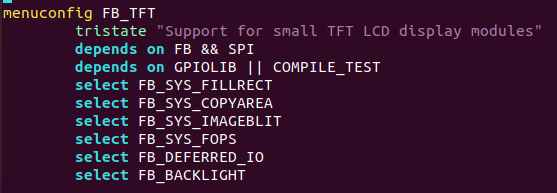
\includegraphics[width=0.5\linewidth]{FB_TFT.png}
                \caption{FB\_TFT}
                \label{fig:fb_tft}
            \end{figure}
            \begin{itemize}
                \item Navigate to \texttt{Device Drivers -> Staging drivers}.
                \item Select \texttt{[*] Support for small TFT display modules}.
            \end{itemize}
            \begin{figure}[H]
                \centering
                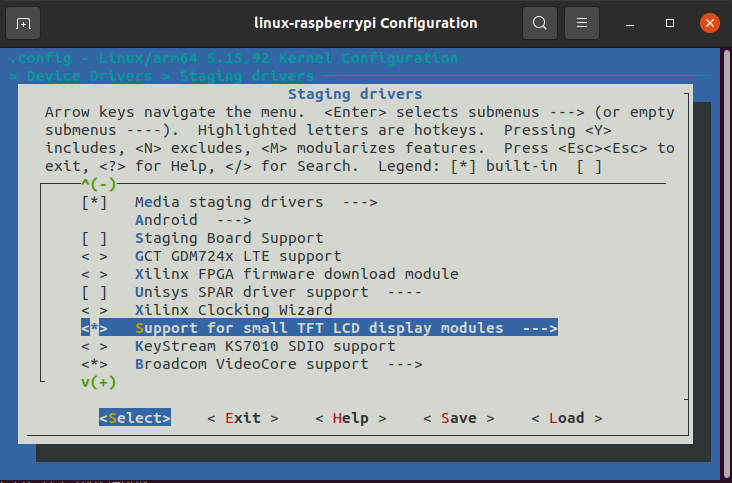
\includegraphics[width=0.5\linewidth]{FB_TFT_menuconfig.png}
                \caption{FB\_TFT menuconfig}
                \label{fig:fb_tft_menuconfig}
            \end{figure}
            
            \item \texttt{\textbf{FB:}}
            \begin{itemize}
                \item Navigate to \texttt{Device Drivers -> Graphics support -> Frame buffer Devices}.
                \item Select \texttt{[*] Support for frame buffer devices}.
            \end{itemize}
            \begin{figure}[H]
                \centering
                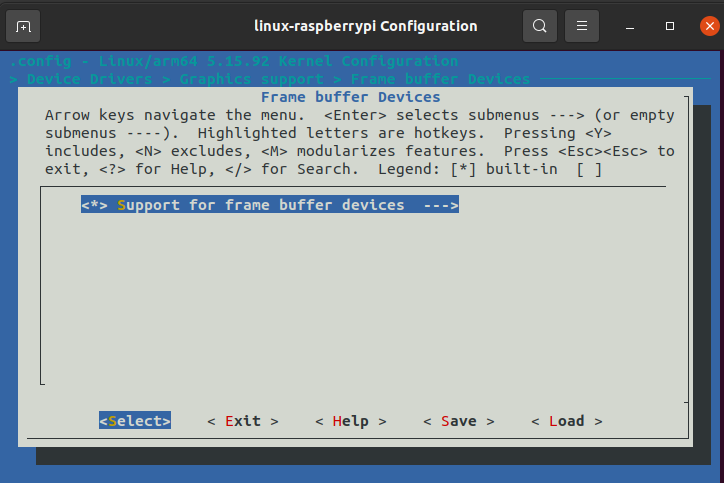
\includegraphics[width=0.5\linewidth]{FB_menuconfig.png}
                \caption{FB menuconfig}
                \label{fig:fb_menuconfig}
            \end{figure}
            
            \item \texttt{\textbf{SPI:}}
            \begin{itemize}
                \item Navigate to \texttt{Device Drivers -> SPI support}.
                \item Select \texttt{[*] BCM2835 SPI controller}.
            \end{itemize}
            \begin{figure}[H]
                \centering
                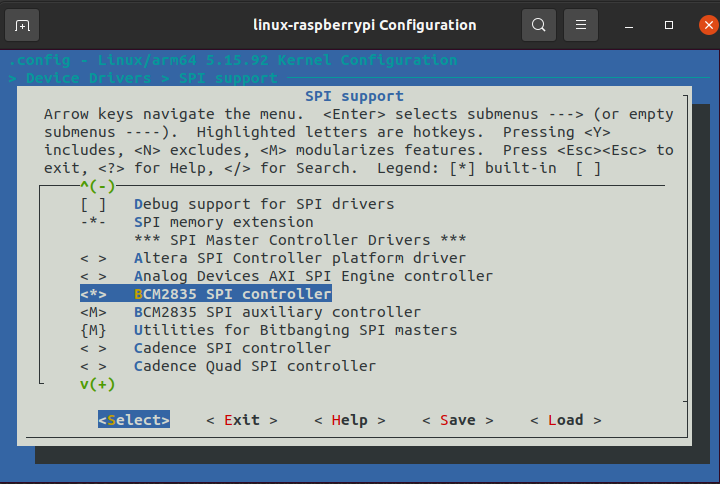
\includegraphics[width=0.5\linewidth]{SPI_menuconfig.png}
                \caption{SPI menuconfig}
                \label{fig:spi_menuconfig}
            \end{figure}
        \end{itemize}
    \end{itemize}

    \item \textbf{Creating and Adding Change Fragments}
    \begin{lstlisting}[language=bash]
    bitbake -c diffconfig virtual/kernel
    \end{lstlisting}
    
    \textbf{Output:}
    \begin{lstlisting}[language=bash]
    Config fragment has been dumped into:
    /home/ngerr/Workspace/LYE_rasp/poky/build/tmp/work/
    raspberrypi4_64-poky-linux/linux-raspberrypi/1_5.15.92+git999-r0/fragment.cfg
    NOTE: Tasks Summary: Attempted 308 tasks of which 307 didn't need to be rerun and all succeeded.
    \end{lstlisting}
    
    \textbf{Fragment Content:}
    \begin{lstlisting}[language=bash]
    CONFIG_SPI_BCM2835=y
    CONFIG_FB_SYS_FILLRECT=y
    CONFIG_FB_SYS_COPYAREA=y
    CONFIG_FB_SYS_IMAGEBLIT=y
    CONFIG_FB_SYS_FOPS=y
    CONFIG_FB_BACKLIGHT=y
    CONFIG_BACKLIGHT_CLASS_DEVICE=y
    CONFIG_FB_TFT=y
    CONFIG_FB_TFT_ILI9341=y
    \end{lstlisting}
    
    \textbf{Adding to Recipe:}
    \begin{lstlisting}[language=bash]
    ls -rlt recipes-kernel/linux/linux-raspberrypi/ili9341_fragment.cfg
    -rw-r--r-- 1 ngerr ngerr 212 Mar 28 23:05 recipes-kernel/linux/linux-raspberrypi/ili9341_fragment.cfg
    \end{lstlisting}
    
    \textbf{Modify .bbappend:}
    \begin{lstlisting}[language=bash]
    SRC_URI += "file://ili9341_fragment.cfg"
    \end{lstlisting}

    \item \textbf{Modify the Device Tree}

    In this section, I'll use \textbf{devtool} to clone the kernel source as a workspace and apply changes. Refer to section 2.4 in \cite{3} for more details.
    
    \begin{itemize}
        \item Step 1: Create the workspace containing the kernel source
        \begin{lstlisting}[language=bash]
        devtool modify linux-raspberrypi
        \end{lstlisting}

        \item Step 2: Modify the \textbf{dts} in the kernel source: \texttt{bcm2711-rpi-4-b.dts}
        
        - Enable the \texttt{\textbf{spi0}} node with \texttt{status = "okay"}.
        - Disable the \texttt{\textbf{spidev0}} node and replace it with a custom node:
        
        \begin{lstlisting}[language=bash]
        diff --git a/arch/arm/boot/dts/bcm2711-rpi-4-b.dts b/arch/arm/boot/dts/bcm2711-rpi-4-b.dts
        index 8c0ab39beea1..e1a654235220 100644
        --- a/arch/arm/boot/dts/bcm2711-rpi-4-b.dts
        +++ b/arch/arm/boot/dts/bcm2711-rpi-4-b.dts
        @@ -327,13 +327,30 @@ &spi0 {
         	pinctrl-names = "default";
         	pinctrl-0 = <&spi0_pins &spi0_cs_pins>;
         	cs-gpios = <&gpio 8 1>, <&gpio 7 1>;
        +	status = "okay";
         
        -	spidev0: spidev@0{
        -		compatible = "spidev";
        -		reg = <0>;
        -		spi-max-frequency = <125000000>;
        +	// spidev0: spidev@0{
        +	// 	compatible = "spidev";
        +	// 	reg = <0>;
        +	// 	spi-max-frequency = <125000000>;
        +	// };
        +	ili9341: LYE_ili9341@0 {
        +		compatible = "ilitek,ili9341";
        +		reg = <0>;
        +		spi-max-frequency = <32000000>;
        +		rotate = <90>;
        +		fps = <60>;
        +		bgr;
        +		buswidth = <8>;
        +		dc-gpios = <&gpio 24 GPIO_ACTIVE_HIGH>;
        +		reset-gpios = <&gpio 25 GPIO_ACTIVE_LOW>;
        +		status = "okay";
         	};
        \end{lstlisting}
        
        \item Save changes and build
        
        - Option 1: Build and test temporarily (refer to step 3-5 in section 2.4 of \cite{3}).
        
        - Option 2: Apply the change permanently to the recipe (refer to step 6-7 in section 2.4 of \cite{3}).

        Example: The custom kernel layer \texttt{meta-kernelmodule} contains the patch:
        
        \begin{figure}[H]
            \centering
            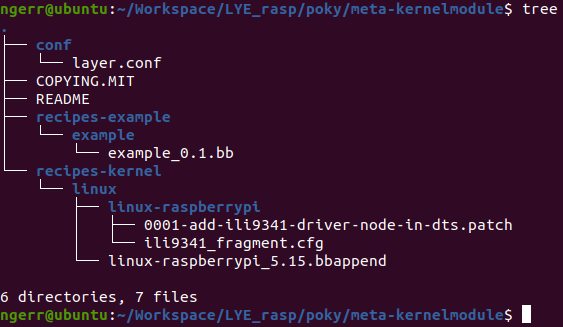
\includegraphics[width=0.5\linewidth]{meta-kernelmodule_tree.png}
            \caption{meta-kernelmodule tree}
        \end{figure}

        \item \texttt{.bbappend} content
        \begin{lstlisting}[language=bash]
        FILESEXTRAPATHS:prepend := "${THISDIR}/${PN}:"

        SRC_URI += "file://0001-add-ili9341-driver-node-in-dts.patch"
        SRC_URI += "file://ili9341_fragment.cfg"
        \end{lstlisting}

    \end{itemize}

    \item \textbf{Check the Result on Hardware}
    \begin{itemize}
        \item \textbf{Wire Connection}
        \begin{figure}[H]
            \centering
            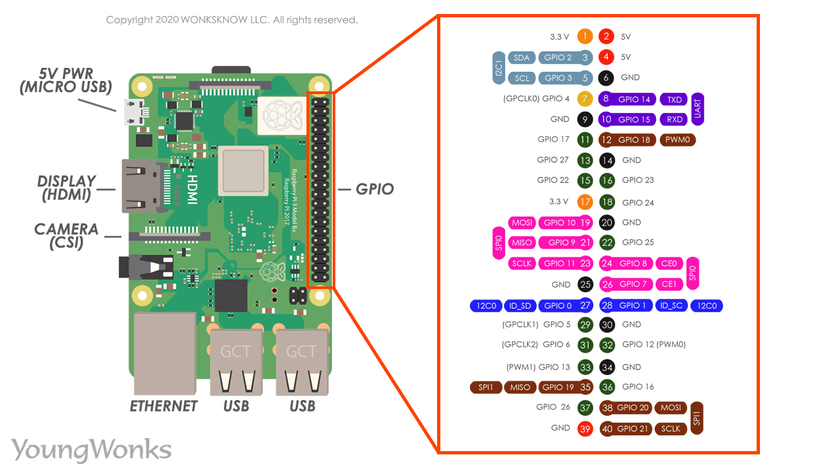
\includegraphics[width=0.5\linewidth]{wire_connection.png}
            \caption{Wire connection}
        \end{figure}
        
        \begin{lstlisting}
        GND  - GND
        VCC  - 3.3V
        CS   - PIN 24 (GPIO 8)
        CLK  - PIN 23 (GPIO 11)
        MOSI - PIN 19 (GPIO 10)
        RES  - PIN 22 (GPIO 25)
        DC   - PIN 18 (GPIO 24)
        LED  - 3.3V
        MISO - (not connected)
        \end{lstlisting}
    
        \item \textbf{Boot Screen}
        \begin{figure}
            \centering
            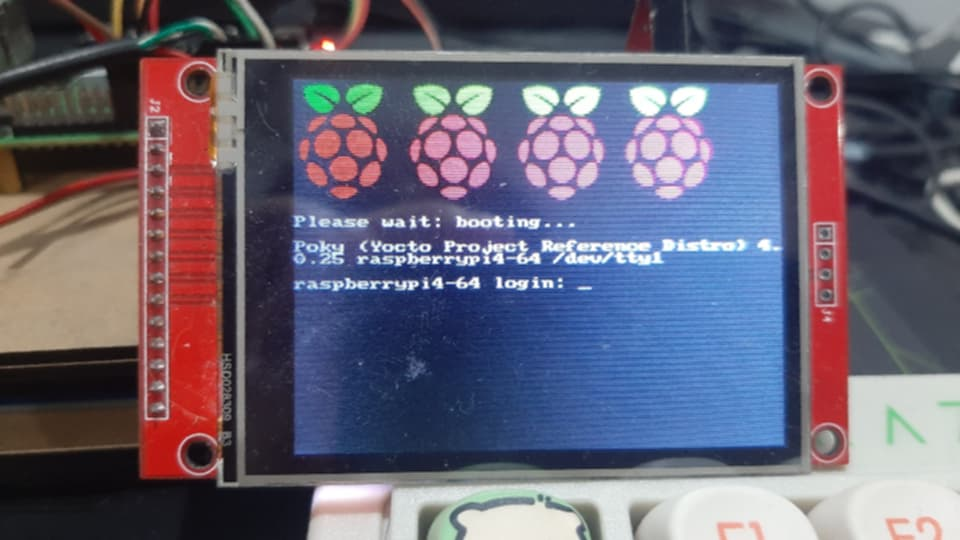
\includegraphics[width=0.5\linewidth]{boot_screen_ili9341.png}
            \caption{ILI9341 Boot Screen}
            \label{fig:enter-label}
        \end{figure}
    \end{itemize}

\end{itemize}


\subsection{I2C}

\subsection{Qt}

\section{Final example to practice} \label{sec:final-example}


\bibliographystyle{plain}
\bibliography{sample}

\end{document}